{
Det vi kalder det gyldne snit, den gyldne ratio eller det guddommelige
forhold, blev allerede beskrevet i Euklids \emph{Elements} fra ca. 300
f.  Kr. som følger:
\begin{quote}
	\emph{``A straight line is said to have been cut in extreme
	and mean ratio when, as the whole line is to the greater
	segment, so is the greater to the less.''}\cite{Euclid300bc}
\end{quote}

\begin{figure}[h!]
	\begin{center}
		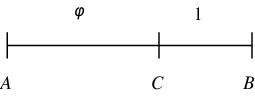
\includegraphics[scale=0.49,angle=0]{afsnit/baggrund/billeder/line_segment_a_c_b}
	\end{center}
	\caption{Euklids opdeling af et linjestykke}
	\label{line_segment}
\end{figure}

Givet et linjestykke $A\ B$, som vist i figur \ref{euclid}, og ud fra
Euklids beskrivelse kan $\varphi$ defineres som
\begin{equation}
	\varphi	= \frac{A\ C}{C\ B} = \frac{A\ B}{A\ C}
	\label{euclid}
\end{equation}
Ved at indsætte variable i ligning \ref{euclid} får vi
\begin{equation}
	\varphi = \frac{\varphi + 1}{\varphi}
	\label{expand_euclid}
\end{equation}
hvilket giver os andengradspolynomiet
\begin{equation}
	\varphi^{2} - \varphi - 1 = 0.
	\label{poly_phi}
\end{equation}
Hvis vi nu løser andengradspolynomiet i ligning \ref{poly_phi}, med
$\varphi > 0$, får vi
\begin{eqnarray*}
	\varphi	& =	& \frac{\sqrt{5} + 1}{2} \\
		& =	& 1.6180\ 3398\ 8749\ 8948\ 4820 \dots
\end{eqnarray*}

Tallet $\varphi$ bemærker sig blandt andet ved, at når det kvadreres, så
lægger man blot 1 til. Dette udledes trivielt fra ligning \ref{poly_phi}
\begin{equation}
	\varphi^{2} = \varphi + 1
	\label{phi_squared}
\end{equation}

Vi kan også finde polynomiets anden rod som angives ved $\varPhi$
\begin{eqnarray*}
	\varPhi & = & \frac{1}{\varphi} \\
		& = & \varphi - 1 \\
		& = & 0.6180\ 3398\ 8749\ 8948\ 4820 \dots 
\end{eqnarray*}
Også tallet $\varPhi$ er interessant idet dets eget kvadrat plus sig
selv giver 1. Vi har at
\begin{equation}
	\varPhi^{2} + \varPhi = 1
	\label{Phi_squared}
\end{equation}
hvilket kun er gældende for $\varPhi$.

Det gyldne snit fremviser endvidere en interessant forbindelse til
Fibonaccis talrække, da forholdet mellem to fibonaccital $F(n)$ og $F(n
- 1)$ konvergerer mod $\varphi$ når $n$ nærmer sig uendelig. Mere
formelt har vi at
\begin{eqnarray*}
	\varphi & =     & \lim_{n \rightarrow
	\infty}{\frac{F(n)}{F(n - 1)}}
\end{eqnarray*}

\subsubsection{Et gyldent rektangel}
På samme måde som vi kan opdele en linjestykke efter det gyldne snit,
kan vi konstruere et rektangel hvor forholdene mellem højde og bredde er
$\varphi$. Vi konstruerer et rektangel hvor alle sider er lig 1 og
tegner en diagonal fra dette rektangelels midte til modsatte hjørne. Med
denne diagonal som radius tegnes en cirkel som et gyldent rektangel kan
tegnes efter. Figur \ref{golden_rectangle} illustrerer denne metode.

\begin{figure}[h!]
	\begin{center}
		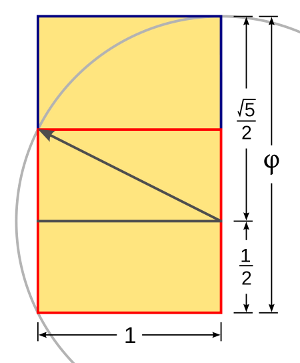
\includegraphics[scale=0.35,angle=0]{afsnit/baggrund/billeder/Golden_Rectangle_Construction}
	\end{center}
	\caption{Et gyldent rektangel - \emph{Kilde: Wikipedia}}
	\label{golden_rectangle}
\end{figure}
Det ses at rektanglet har forholdet $\varphi:1$ og at eksemplet er helt
analogt til det linjestykke givet i figur \ref{line_segment}. Dog skal
det bemærkes, at det rektangel der kan konstrueres af linjestykkerne 1
og $\varphi - 1$ også er et gyldent rektangel med forholdet $1:\varphi
-1 = \varphi$. Man kan derved konstruere gyldne rektangler ud i det
uendelige ved hele tiden at lave nye gyldne rektangler.

\subsubsection{Spiraler og det gyldne snit}
Når man som ovenfor, gentagende gange deler et gyldent rektangel kan man
bruge dette til at konstruere en gylden spiral. En gylden spiral kan
skrives ved ligningen for generelle logaritmiske spiraler som
\begin{equation}
	r = ae^{c\theta}
	\label{log_spiral_2}
\end{equation}
eller
\begin{equation}
	\theta = \frac{1}{c}\ln(r/a)
	\label{log_spiral_1}
\end{equation}
hvor $e$ er grundtallet for den naturlige logaritme og $c$ skal have en
speciel værdi for at kunne være en gylden spiral. Den gyldne spiral kan
approksimeres ved at konstruere en fibonaccispiral som vist i figur
\ref{fibonacci_spiral}.
\begin{figure}[h!]
	\begin{center}
		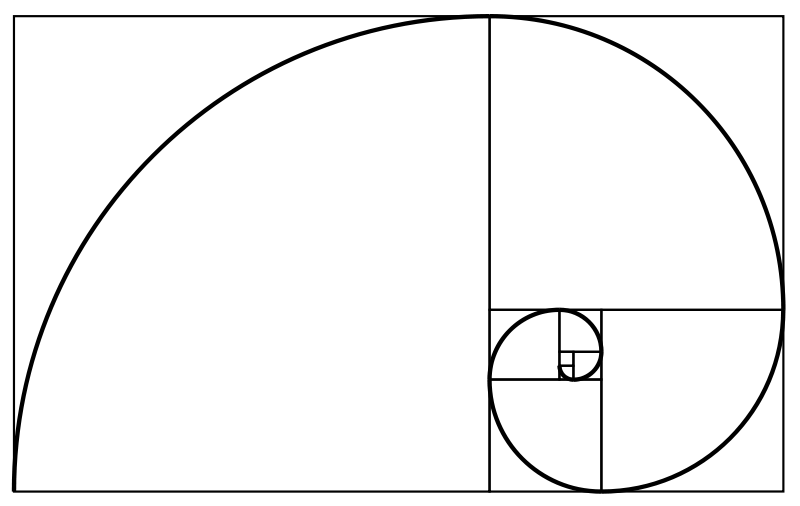
\includegraphics[scale=0.35,angle=0]{afsnit/baggrund/billeder/Fibonacci_spiral}
	\end{center}
	\caption{En fibonaccispiral - \emph{Kilde: Wikipedia}}
	\label{fibonacci_spiral}
\end{figure}
Da fibonaccispiralen er konstrueret efter Fibonaccis talrække nærmer
denne spiral sig en gylden spiral, men kan ikke betegnes som værende en
ægte gylden spiral.

Med den matematiske definition på plads kan vi kigge på den forskning
der er blevet gjort i forbindelse med det gyldne snit.

% vim: set tw=72 spell spelllang=da:
